% Generated by Sphinx.
\def\sphinxdocclass{article}
\documentclass[letterpaper,10pt,english]{sphinxhowto}
\usepackage[utf8]{inputenc}
\DeclareUnicodeCharacter{00A0}{\nobreakspace}
\usepackage[T1]{fontenc}
\usepackage{babel}
\usepackage{times}
\usepackage[Bjarne]{fncychap}
\usepackage{longtable}
\usepackage{sphinx}
\usepackage{multirow}
\usepackage{color}
\makeatletter
\renewenvironment{notice}[2]{
\begin{itshape}}{\end{itshape}}
\makeatother

\usepackage{letltxmacro}

% save the meaning of \includegraphics
\LetLtxMacro\latexhreffoot\href
\renewcommand{\href}[2]{%
\latexhreffoot{#1}{#2\footnote{\url{#1}}}}

\definecolor{light-gray}{gray}{0.95}
\title{Siren Demo at SIGMOD 2014}
\date{June, 2014}
\release{2.1.1}
\author{Esther Galbrun and Pauli Miettinen}
\newcommand{\sphinxlogo}{}
\renewcommand{\releasename}{Release}
\makeindex

\makeatletter
\def\PYG@reset{\let\PYG@it=\relax \let\PYG@bf=\relax%
    \let\PYG@ul=\relax \let\PYG@tc=\relax%
    \let\PYG@bc=\relax \let\PYG@ff=\relax}
\def\PYG@tok#1{\csname PYG@tok@#1\endcsname}
\def\PYG@toks#1+{\ifx\relax#1\empty\else%
    \PYG@tok{#1}\expandafter\PYG@toks\fi}
\def\PYG@do#1{\PYG@bc{\PYG@tc{\PYG@ul{%
    \PYG@it{\PYG@bf{\PYG@ff{#1}}}}}}}
\def\PYG#1#2{\PYG@reset\PYG@toks#1+\relax+\PYG@do{#2}}

\expandafter\def\csname PYG@tok@gd\endcsname{\def\PYG@tc##1{\textcolor[rgb]{0.63,0.00,0.00}{##1}}}
\expandafter\def\csname PYG@tok@gu\endcsname{\let\PYG@bf=\textbf\def\PYG@tc##1{\textcolor[rgb]{0.50,0.00,0.50}{##1}}}
\expandafter\def\csname PYG@tok@gt\endcsname{\def\PYG@tc##1{\textcolor[rgb]{0.00,0.27,0.87}{##1}}}
\expandafter\def\csname PYG@tok@gs\endcsname{\let\PYG@bf=\textbf}
\expandafter\def\csname PYG@tok@gr\endcsname{\def\PYG@tc##1{\textcolor[rgb]{1.00,0.00,0.00}{##1}}}
\expandafter\def\csname PYG@tok@cm\endcsname{\let\PYG@it=\textit\def\PYG@tc##1{\textcolor[rgb]{0.25,0.50,0.56}{##1}}}
\expandafter\def\csname PYG@tok@vg\endcsname{\def\PYG@tc##1{\textcolor[rgb]{0.73,0.38,0.84}{##1}}}
\expandafter\def\csname PYG@tok@m\endcsname{\def\PYG@tc##1{\textcolor[rgb]{0.13,0.50,0.31}{##1}}}
\expandafter\def\csname PYG@tok@mh\endcsname{\def\PYG@tc##1{\textcolor[rgb]{0.13,0.50,0.31}{##1}}}
\expandafter\def\csname PYG@tok@cs\endcsname{\def\PYG@tc##1{\textcolor[rgb]{0.25,0.50,0.56}{##1}}\def\PYG@bc##1{\setlength{\fboxsep}{0pt}\colorbox[rgb]{1.00,0.94,0.94}{\strut ##1}}}
\expandafter\def\csname PYG@tok@ge\endcsname{\let\PYG@it=\textit}
\expandafter\def\csname PYG@tok@vc\endcsname{\def\PYG@tc##1{\textcolor[rgb]{0.73,0.38,0.84}{##1}}}
\expandafter\def\csname PYG@tok@il\endcsname{\def\PYG@tc##1{\textcolor[rgb]{0.13,0.50,0.31}{##1}}}
\expandafter\def\csname PYG@tok@go\endcsname{\def\PYG@tc##1{\textcolor[rgb]{0.20,0.20,0.20}{##1}}}
\expandafter\def\csname PYG@tok@cp\endcsname{\def\PYG@tc##1{\textcolor[rgb]{0.00,0.44,0.13}{##1}}}
\expandafter\def\csname PYG@tok@gi\endcsname{\def\PYG@tc##1{\textcolor[rgb]{0.00,0.63,0.00}{##1}}}
\expandafter\def\csname PYG@tok@gh\endcsname{\let\PYG@bf=\textbf\def\PYG@tc##1{\textcolor[rgb]{0.00,0.00,0.50}{##1}}}
\expandafter\def\csname PYG@tok@ni\endcsname{\let\PYG@bf=\textbf\def\PYG@tc##1{\textcolor[rgb]{0.84,0.33,0.22}{##1}}}
\expandafter\def\csname PYG@tok@nl\endcsname{\let\PYG@bf=\textbf\def\PYG@tc##1{\textcolor[rgb]{0.00,0.13,0.44}{##1}}}
\expandafter\def\csname PYG@tok@nn\endcsname{\let\PYG@bf=\textbf\def\PYG@tc##1{\textcolor[rgb]{0.05,0.52,0.71}{##1}}}
\expandafter\def\csname PYG@tok@no\endcsname{\def\PYG@tc##1{\textcolor[rgb]{0.38,0.68,0.84}{##1}}}
\expandafter\def\csname PYG@tok@na\endcsname{\def\PYG@tc##1{\textcolor[rgb]{0.25,0.44,0.63}{##1}}}
\expandafter\def\csname PYG@tok@nb\endcsname{\def\PYG@tc##1{\textcolor[rgb]{0.00,0.44,0.13}{##1}}}
\expandafter\def\csname PYG@tok@nc\endcsname{\let\PYG@bf=\textbf\def\PYG@tc##1{\textcolor[rgb]{0.05,0.52,0.71}{##1}}}
\expandafter\def\csname PYG@tok@nd\endcsname{\let\PYG@bf=\textbf\def\PYG@tc##1{\textcolor[rgb]{0.33,0.33,0.33}{##1}}}
\expandafter\def\csname PYG@tok@ne\endcsname{\def\PYG@tc##1{\textcolor[rgb]{0.00,0.44,0.13}{##1}}}
\expandafter\def\csname PYG@tok@nf\endcsname{\def\PYG@tc##1{\textcolor[rgb]{0.02,0.16,0.49}{##1}}}
\expandafter\def\csname PYG@tok@si\endcsname{\let\PYG@it=\textit\def\PYG@tc##1{\textcolor[rgb]{0.44,0.63,0.82}{##1}}}
\expandafter\def\csname PYG@tok@s2\endcsname{\def\PYG@tc##1{\textcolor[rgb]{0.25,0.44,0.63}{##1}}}
\expandafter\def\csname PYG@tok@vi\endcsname{\def\PYG@tc##1{\textcolor[rgb]{0.73,0.38,0.84}{##1}}}
\expandafter\def\csname PYG@tok@nt\endcsname{\let\PYG@bf=\textbf\def\PYG@tc##1{\textcolor[rgb]{0.02,0.16,0.45}{##1}}}
\expandafter\def\csname PYG@tok@nv\endcsname{\def\PYG@tc##1{\textcolor[rgb]{0.73,0.38,0.84}{##1}}}
\expandafter\def\csname PYG@tok@s1\endcsname{\def\PYG@tc##1{\textcolor[rgb]{0.25,0.44,0.63}{##1}}}
\expandafter\def\csname PYG@tok@gp\endcsname{\let\PYG@bf=\textbf\def\PYG@tc##1{\textcolor[rgb]{0.78,0.36,0.04}{##1}}}
\expandafter\def\csname PYG@tok@sh\endcsname{\def\PYG@tc##1{\textcolor[rgb]{0.25,0.44,0.63}{##1}}}
\expandafter\def\csname PYG@tok@ow\endcsname{\let\PYG@bf=\textbf\def\PYG@tc##1{\textcolor[rgb]{0.00,0.44,0.13}{##1}}}
\expandafter\def\csname PYG@tok@sx\endcsname{\def\PYG@tc##1{\textcolor[rgb]{0.78,0.36,0.04}{##1}}}
\expandafter\def\csname PYG@tok@bp\endcsname{\def\PYG@tc##1{\textcolor[rgb]{0.00,0.44,0.13}{##1}}}
\expandafter\def\csname PYG@tok@c1\endcsname{\let\PYG@it=\textit\def\PYG@tc##1{\textcolor[rgb]{0.25,0.50,0.56}{##1}}}
\expandafter\def\csname PYG@tok@kc\endcsname{\let\PYG@bf=\textbf\def\PYG@tc##1{\textcolor[rgb]{0.00,0.44,0.13}{##1}}}
\expandafter\def\csname PYG@tok@c\endcsname{\let\PYG@it=\textit\def\PYG@tc##1{\textcolor[rgb]{0.25,0.50,0.56}{##1}}}
\expandafter\def\csname PYG@tok@mf\endcsname{\def\PYG@tc##1{\textcolor[rgb]{0.13,0.50,0.31}{##1}}}
\expandafter\def\csname PYG@tok@err\endcsname{\def\PYG@bc##1{\setlength{\fboxsep}{0pt}\fcolorbox[rgb]{1.00,0.00,0.00}{1,1,1}{\strut ##1}}}
\expandafter\def\csname PYG@tok@kd\endcsname{\let\PYG@bf=\textbf\def\PYG@tc##1{\textcolor[rgb]{0.00,0.44,0.13}{##1}}}
\expandafter\def\csname PYG@tok@ss\endcsname{\def\PYG@tc##1{\textcolor[rgb]{0.32,0.47,0.09}{##1}}}
\expandafter\def\csname PYG@tok@sr\endcsname{\def\PYG@tc##1{\textcolor[rgb]{0.14,0.33,0.53}{##1}}}
\expandafter\def\csname PYG@tok@mo\endcsname{\def\PYG@tc##1{\textcolor[rgb]{0.13,0.50,0.31}{##1}}}
\expandafter\def\csname PYG@tok@mi\endcsname{\def\PYG@tc##1{\textcolor[rgb]{0.13,0.50,0.31}{##1}}}
\expandafter\def\csname PYG@tok@kn\endcsname{\let\PYG@bf=\textbf\def\PYG@tc##1{\textcolor[rgb]{0.00,0.44,0.13}{##1}}}
\expandafter\def\csname PYG@tok@o\endcsname{\def\PYG@tc##1{\textcolor[rgb]{0.40,0.40,0.40}{##1}}}
\expandafter\def\csname PYG@tok@kr\endcsname{\let\PYG@bf=\textbf\def\PYG@tc##1{\textcolor[rgb]{0.00,0.44,0.13}{##1}}}
\expandafter\def\csname PYG@tok@s\endcsname{\def\PYG@tc##1{\textcolor[rgb]{0.25,0.44,0.63}{##1}}}
\expandafter\def\csname PYG@tok@kp\endcsname{\def\PYG@tc##1{\textcolor[rgb]{0.00,0.44,0.13}{##1}}}
\expandafter\def\csname PYG@tok@w\endcsname{\def\PYG@tc##1{\textcolor[rgb]{0.73,0.73,0.73}{##1}}}
\expandafter\def\csname PYG@tok@kt\endcsname{\def\PYG@tc##1{\textcolor[rgb]{0.56,0.13,0.00}{##1}}}
\expandafter\def\csname PYG@tok@sc\endcsname{\def\PYG@tc##1{\textcolor[rgb]{0.25,0.44,0.63}{##1}}}
\expandafter\def\csname PYG@tok@sb\endcsname{\def\PYG@tc##1{\textcolor[rgb]{0.25,0.44,0.63}{##1}}}
\expandafter\def\csname PYG@tok@k\endcsname{\let\PYG@bf=\textbf\def\PYG@tc##1{\textcolor[rgb]{0.00,0.44,0.13}{##1}}}
\expandafter\def\csname PYG@tok@se\endcsname{\let\PYG@bf=\textbf\def\PYG@tc##1{\textcolor[rgb]{0.25,0.44,0.63}{##1}}}
\expandafter\def\csname PYG@tok@sd\endcsname{\let\PYG@it=\textit\def\PYG@tc##1{\textcolor[rgb]{0.25,0.44,0.63}{##1}}}

\def\PYGZbs{\char`\\}
\def\PYGZus{\char`\_}
\def\PYGZob{\char`\{}
\def\PYGZcb{\char`\}}
\def\PYGZca{\char`\^}
\def\PYGZam{\char`\&}
\def\PYGZlt{\char`\<}
\def\PYGZgt{\char`\>}
\def\PYGZsh{\char`\#}
\def\PYGZpc{\char`\%}
\def\PYGZdl{\char`\$}
\def\PYGZhy{\char`\-}
\def\PYGZsq{\char`\'}
\def\PYGZdq{\char`\"}
\def\PYGZti{\char`\~}
% for compatibility with earlier versions
\def\PYGZat{@}
\def\PYGZlb{[}
\def\PYGZrb{]}
\makeatother

\begin{document}
\maketitle
\vspace{-15em}

\includegraphics[width=0.2\textwidth]{siren_icon.png}

\vspace{20em}
\vfill
\phantomsection\label{index::doc}

% 
\begin{center}
%\colorbox{light-gray}{\parbox[c][10em][c]{0.85\textwidth}{
\begin{center}
\begin{notice}{note}{Note:}
This document summarizes information about the demonstration of the \emph{Siren} interactive interface for redescription mining presented at the \href{http://sigmod2014.org}{2014 ACM SIGMOD/PODS Conference, Snowbird, Utah, USA on June 22-27, 2014.}

\bigskip{}

Esther Galbrun and Pauli Miettinen. Interactive Redescription Mining. In \emph{SIGMOD}. 2014.

\bigskip{}

More details can be found on the main \emph{Siren} \href{http://www.cs.helsinki.fi/u/galbrun/redescriptors/siren/main/}{webpage} or in the \href{http://www.cs.helsinki.fi/u/galbrun/redescriptors/siren/help/}{user guide.}
\end{notice}
\end{center}
%}}
\end{center}
% 

\vspace{5em}
\vfill
{\large
%\begin{center}
Redescription mining is a powerful data analysis tool that aims at finding alternative descriptions of the same entities.

%\begin{center}
For example, in biology, an important task is to identify the bioclimatic constraints that allow some species to survive, that is, to describe geographical regions in terms of both their bioclimatic conditions and the fauna that inhabit them.
%\end{center}

%\begin{flushright}
\emph{Siren} is a tool for interactive mining and visualization of redescriptions.\\ It is based on the ReReMi mining algorithm. 
%\end{flushright}
%\end{center}
}
%}
\vfill
~
\newpage
~
\vfill


\section{Download}
\label{download:introduction}\label{download:download}\label{download:intro}\label{download::doc}\label{download:id1}
\emph{Siren} is a multi-platform software.
\emph{Siren} and it's core mining algorithm \emph{ReReMi} are implemented in Python.
It has been used on MacOS and Ubuntu Linux.

Siren and ReReMi are licensed under the Apache License, Version 2.0.
\begin{itemize}
\item {} 
\textbf{Source code} (packaged using Python distutils)\footnote{\url{http://www.cs.helsinki.fi/u/galbrun/redescriptors/code/siren/python-siren-2.1.1.tar.gz}}

\item {} 
\textbf{OS X}\footnote{\url{http://www.cs.helsinki.fi/u/pamietti/data/siren/Siren\_2\_1\_1.dmg}}

\item {} 
\textbf{Linux} (deb)\footnote{\url{http://www.cs.helsinki.fi/u/galbrun/redescriptors/code/siren/python-siren\_2.1.1\_all.deb}}

\item {} 
\textbf{Windows}  (installation executable)\footnote{\url{http://www.cs.helsinki.fi/u/galbrun/redescriptors/code/siren/install\_siren\_2.1.1.exe}}

\end{itemize}



\section{Data Formats}
\label{formats:data-formats}\label{formats::doc}\label{formats:formats}
In \emph{Siren}, data include:
\begin{itemize}
\item {} 
\textbf{Variables}: The variables describing the entities are divided in two sets. They can be of three types:
\begin{enumerate}
\item {} 
Boolean,

\item {} 
categorical,

\item {} 
or real-valued.

\end{enumerate}

\end{itemize}

Obviously, this is required.
\begin{itemize}
\item {} 
\textbf{Entities names}: Optional additional information, providing names for the entities.

\item {} 
\textbf{Variable names}: Optional additional information, providing names for the variables.

\item {} 
\textbf{Coordinates}: Optional location information, i.e. geographic coordinates of the entities. This makes the data geospatial.

\end{itemize}

Data can be imported to \emph{Siren} via the interface menu \emph{File \(\rightarrow\) Import \(\rightarrow\) Import Data}.

Data can be imported into \emph{Siren} as CSV files. The program expects a pair of files, one for either side in character-separated values, as can be imported and exported to and from spreadsheet programms, for instance.

In particular, the data can stored as a table with one column for each variable and one row each entity.
The first row can contain the names of the variables.
The entities names can be included as columns named \emph{ids}. Similarly the coordinates can be included as a pair of columns named \emph{longitudes} and \emph{latitudes}, respectively.


\vfill
~
\newpage
~
\vfill

\section{Functionalities}
\label{functionalities::doc}\label{functionalities:functionalities}\label{functionalities:funct}
Using \emph{Siren}, a user can explore data of his interest by interactively mining, visualizing and editing redescriptions.


\subsection{Mining}
\label{functionalities:mining}\label{functionalities:func-mine}
At the core of \emph{Siren} is the \emph{ReReMi} redescription
mining algorithm. Various modes of interaction with the mining
algorithm are possible through the interface.
\begin{itemize}
\item {} 
Mine redescriptions from the data automatically.

\item {} 
Mine extensions of an existing redescription, on both sides or selectively on one side.

\item {} 
It is possible to select a subset of variables for use in mining/expanding, by disabling some variables and to specify a subset of entities of interest to emphasize.

\end{itemize}


\subsection{Vizualizing}
\label{functionalities:vizualizing}\label{functionalities:func-viz}
\emph{Siren} offers a number of different visualizations.
\begin{itemize}
\item A \emph{parallel coordinates} plot represents the values taken by the entites for the variable appearing in the queries. It allows to easily visualize the impact of the queries conditions on the support of the redescription.
\item A number of \emph{data projections} from the scikit-learn package allow to highlight different aspects of the data.
\item A \emph{map} (for geospatial data) to show the locations where both queries hold, only the left hand side query
holds and only the right hand side query holds.
\end{itemize}

\begin{figure}[h]
\begin{tabular}{cc}
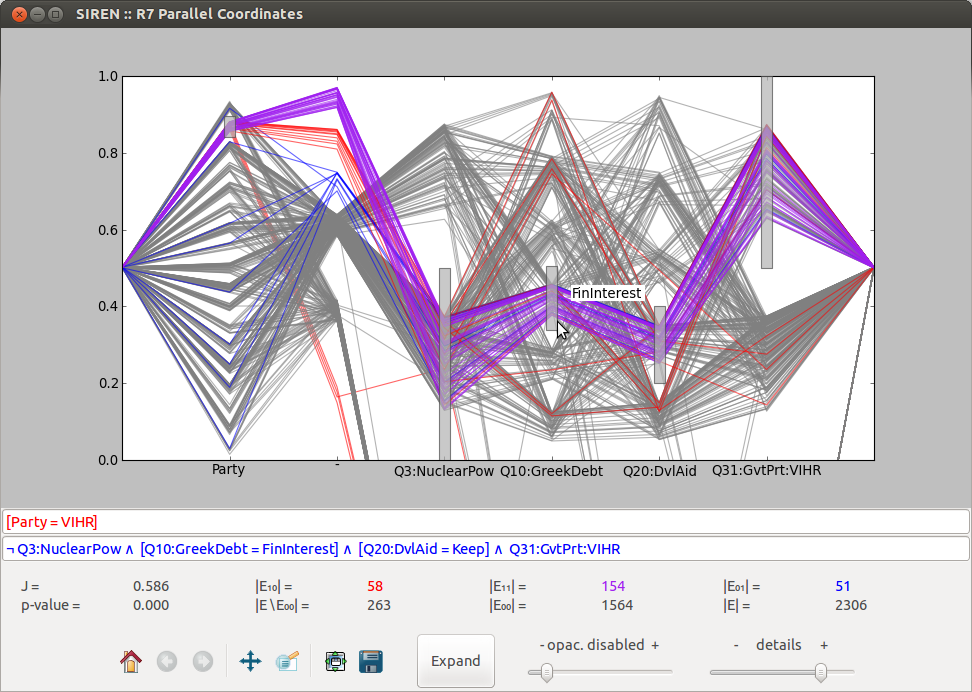
\includegraphics[height=15em]{Siren_vaalikone_para.png} &
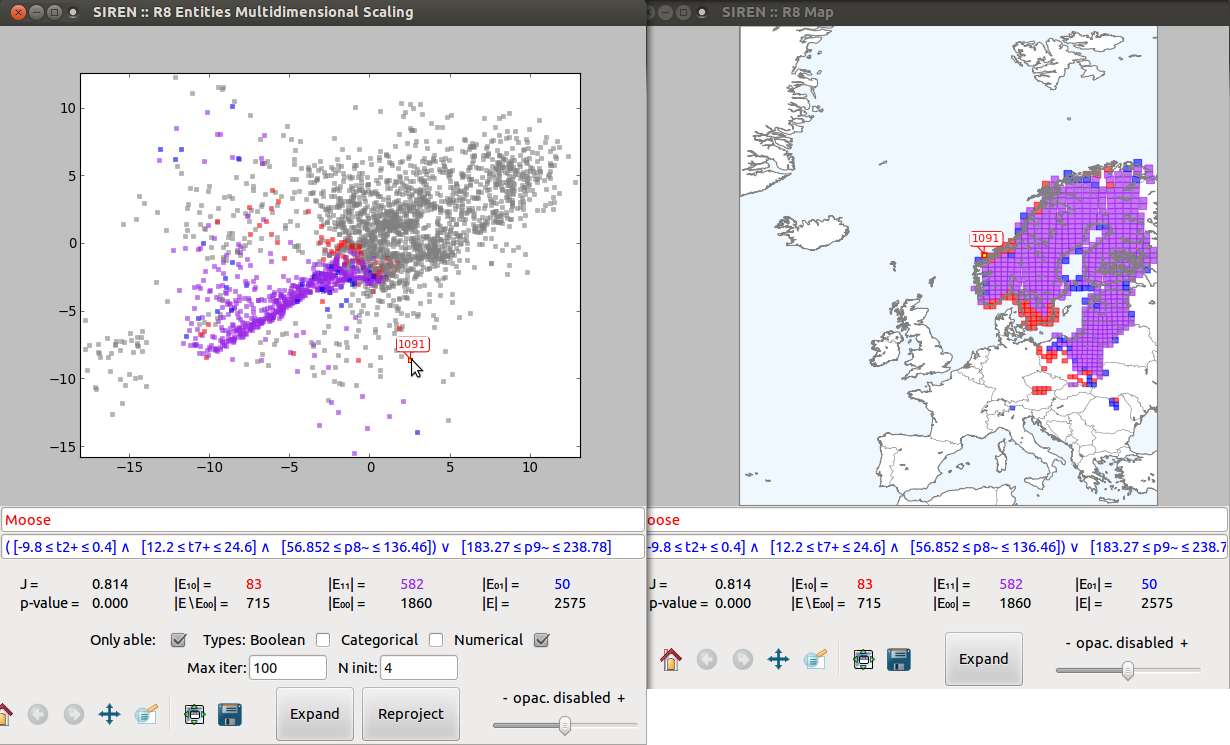
\includegraphics[height=15em]{Bio_SelectDotSideRMoose} \\
\end{tabular}
\end{figure}

\subsection{Editing and Selecting}
\label{functionalities:editing-and-selecting}\label{functionalities:func-edit}
Existing redescriptions can be edited and the visualization and statistics will automatically recomputed.
It is also possible to build a new redescription from scratch.

\vfill
~
\newpage
~
\vfill

\section{Sample Use-Cases}
\label{use_cases:sample-use-cases}\label{use_cases:usecase}\label{use_cases::doc}

\subsection{Finnish 2011 parliamentary elections}
\label{use_cases:finnish-2011-parliamentary-elections}\label{use_cases:uc-finnelec}
We provide a prepared dataset about the Finnish 2011 parliamentary elections. Get the data (non-geospatial), try out \emph{Siren} and learn about the finnish political scene! (More details on the main webpage.)

To illustrate the use of \emph{Siren}, we present example use-cases from different application domains.


\subsection{Biological niche-finding}
\label{use_cases:biological-niche-finding}\label{use_cases:uc-bio}
One use-case concerns niche-finding, i.e. the problem of finding species' bioclimatic envelope, an important task in biology.

\subsection{DBLP Computer Science Bibliography}
\label{use_cases:dblp-computer-science-bibliography}\label{use_cases:uc-dblp}
We also consider non-geospatial data, namely from the DBLP Computer Science Bibliography.

\bigskip{}
\section{Resources}
\label{references:references}\label{references::doc}\label{references:resources}
\begin{thebibliography}{A}
\bibitem[A]{A}{\phantomsection\label{references:a} 
Esther Galbrun and Pauli Miettinen. A Case of Visual and Interactive Data Analysis: Geospatial Redescription Mining. In \emph{Instant Interactive Data Mining Workshop @ ECML-PKDD}. 2012.
}
\bibitem[B]{B}{\phantomsection\label{references:b} 
Esther Galbrun and Pauli Miettinen. Siren: an interactive tool for mining and visualizing geospatial redescriptions. In \emph{KDD}, 1544–1547. ACM, 2012.
}
\bibitem[C]{C}{\phantomsection\label{references:c} 
Esther Galbrun and Pauli Miettinen. From black and white to full color: extending redescription mining outside the Boolean world. \emph{Statistical Analysis and Data Mining}, 5(4):284–303, 2012.
}
\bibitem[D]{D}{\phantomsection\label{references:d} 
Esther Galbrun and Pauli Miettinen. From Black and White to Full Colour: Extending Redescription Mining Outside the Boolean World. In \emph{SDM}, 546–557. 2011.
}
\bibitem[E]{E}{\phantomsection\label{references:e} 
Esther Galbrun. Methods for Redescription Mining. PhD thesis, University of Helsinki, 2014. \url{http://urn.fi/URN:ISBN:978-952-10-9431-6}
}
\end{thebibliography}
\vfill
~
\end{document}
